\documentclass[french,a4paper,10pt]{article}
% pdflatex compte_rendu.tex -output-directory=out && mv out/compte_rendu.pdf ./

\usepackage[a4paper,hmargin=30mm,vmargin=30mm]{geometry}
\usepackage[T1]{fontenc} % font type
\usepackage[french]{babel} % language
\usepackage{lmodern} % font type
\usepackage[shortlabels]{enumitem}
\usepackage{hyperref}
\usepackage{graphicx}
\usepackage{sectsty}
\usepackage{amsmath}
%\setlength{\parindent}{0pt}



\title{Compte Rendu TP noté}
\author{Ivan Lejeune}
\date{\today}


\begin{document}
    \maketitle

    % make table of contents
    \tableofcontents

    \newpage
   
    \section{Transformation de l'espace RGB vers l'espace YCbCr}\label{sec:1}

    \subsection{Choix de l'image}\label{subsec:1.1}

    On utilise l'image \texttt{kodim04\_Red\_Riding\_Hood.ppm} qui correspond à :

    \begin{figure}[!htb]
        \begin{minipage}{0.48\textwidth}
            \centering
            \fbox{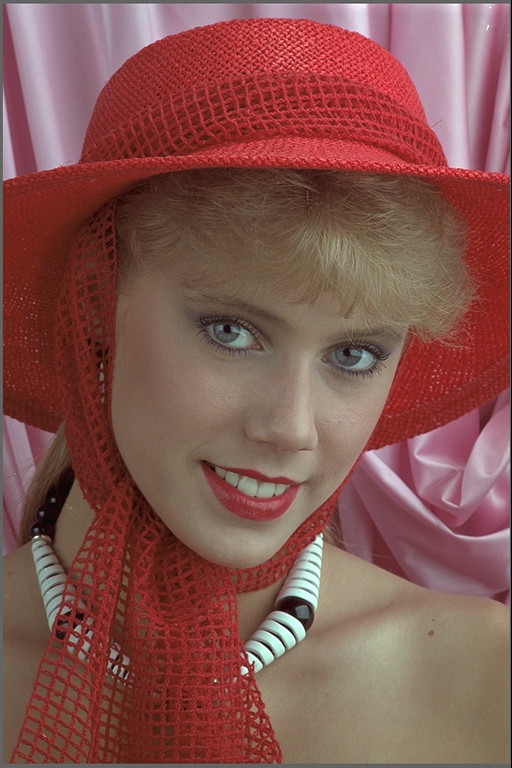
\includegraphics[width=.7\linewidth]{./out/kodim04_Red_Riding_Hood}}
            \caption{Composante Y}\label{Fig:peppers_y}
        \end{minipage}\hfill
    \end{figure}

    On obtient alors les résultats suivants :
    % insert peppers-y, peppers-cb, peppers-cr
    \begin{figure}[!htb]
        \begin{minipage}{0.3\textwidth}
            \centering
            \fbox{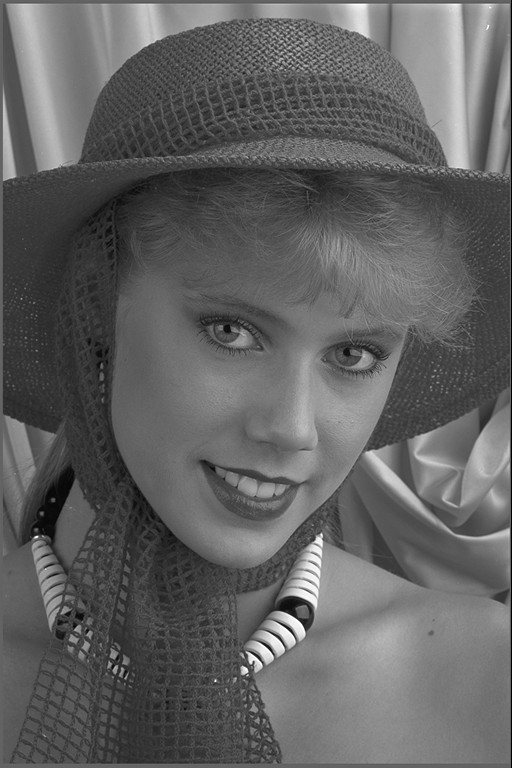
\includegraphics[width=.7\linewidth]{./out/kodim04_Red_Riding_Hood_Y}}
            \caption{Composante Y}\label{Fig:peppers_y}
        \end{minipage}\hfill
        \begin{minipage}{0.3\textwidth}
            \centering
            \fbox{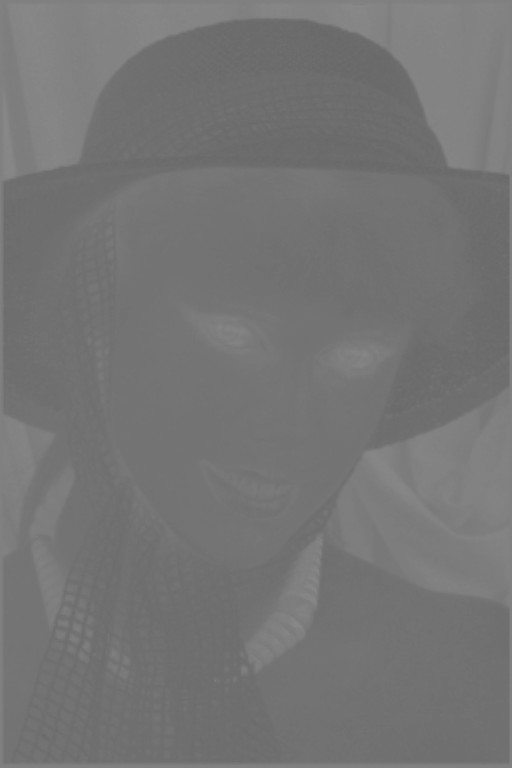
\includegraphics[width=.7\linewidth]{./out/kodim04_Red_Riding_Hood_Cb}}
            \caption{Composante Cb}\label{Fig:peppers_cb}
        \end{minipage}\hfill
        \begin{minipage}{0.3\textwidth}
            \centering
            \fbox{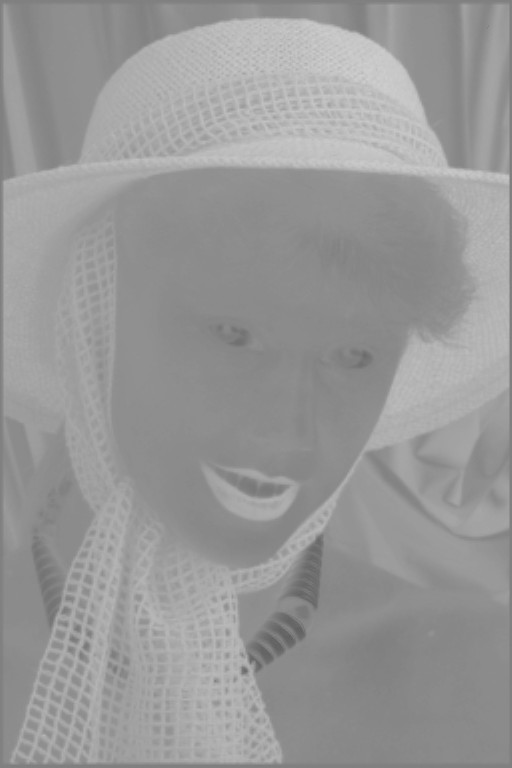
\includegraphics[width=.7\linewidth]{./out/kodim04_Red_Riding_Hood_Cr}}
            \caption{Composante Cr}\label{Fig:peppers_cr}
        \end{minipage}
    \end{figure}

    L'histogramme obtenu correspond à :

    \begin{figure}[!htb]
        \begin{minipage}{0.48\textwidth}
            \centering
            \fbox{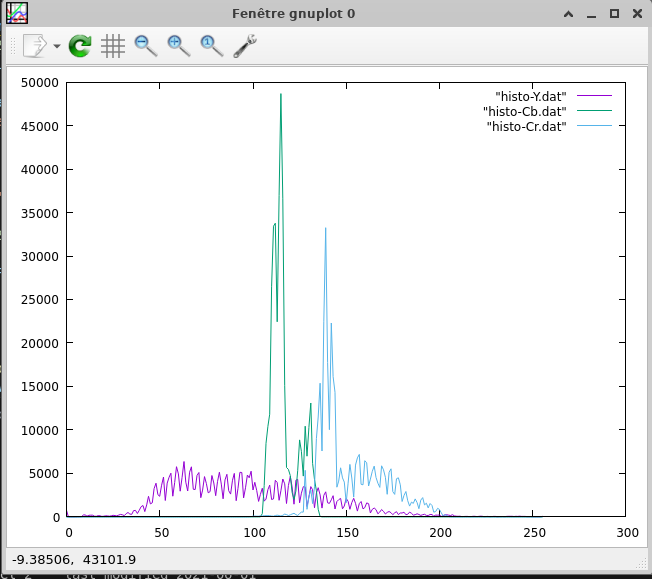
\includegraphics[width=.7\linewidth]{./out/histo-kodim}}
            \caption{Histogramme des composantes}\label{Fig:peppers_y}
        \end{minipage}\hfill
    \end{figure}

    On peut voir ici sur l'histogramme que la partie \texttt{Y} a une grande repartition de niveaux
    de gris alors que les parties \texttt{Cb} et \texttt{Cb} ont une plus grande concentration de
    niveaux restreints.

    \newpage

    \section{Densité de probabilité d'une image}\label{sec:2}

    On obtient l'histogramme suivant :
    % insert orig-peppers and peppers-rgb
    \begin{figure}[!htb]
        \begin{minipage}{0.48\textwidth}
            \centering
            \fbox{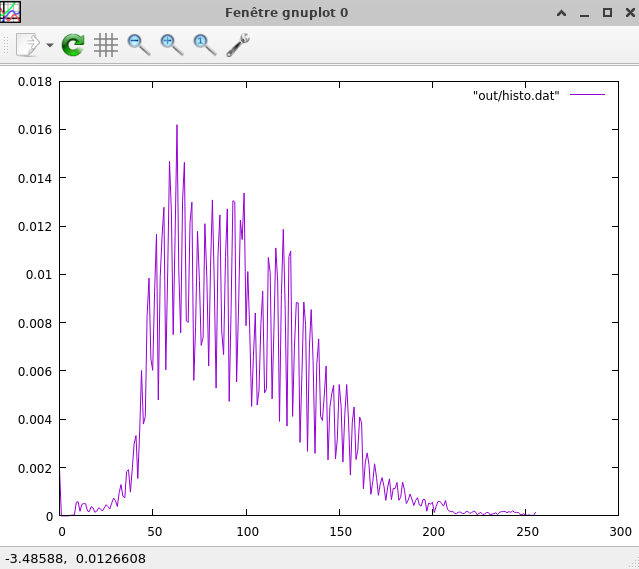
\includegraphics[width=.7\linewidth]{./out/histo-ddp}}
            \caption{Densité de probabilité}\label{Fig:orig-peppers-4}
        \end{minipage}\hfill
    \end{figure}

    On constante qu'il y a une grande variance de concentration et que cela ressemble
    à une courbe gaussienne et donc une répartition particulière.

    \newpage
    \section{Fonction de répartition}\label{sec:3}

    On obtient l'histogramme suivant :
    % insert orig-peppers and peppers-rgb
    \begin{figure}[!htb]
        \begin{minipage}{0.48\textwidth}
            \centering
            \fbox{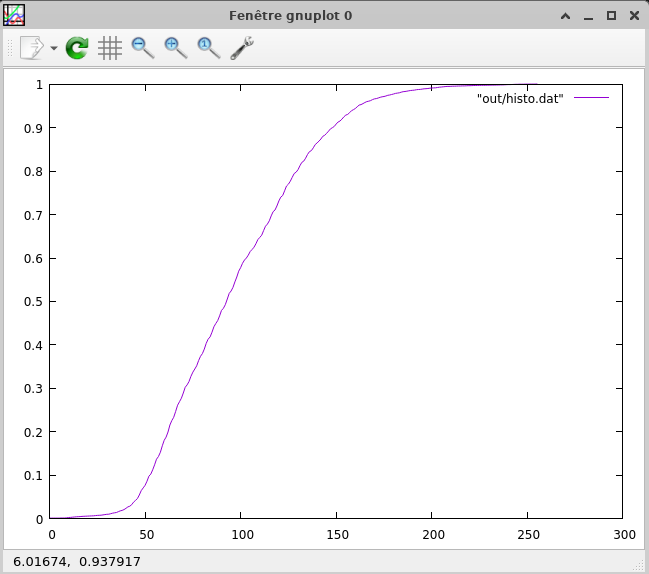
\includegraphics[width=.7\linewidth]{./out/histo-repartition}}
            \caption{Fonction de répartition}\label{Fig:orig-peppers-3}
        \end{minipage}\hfill
    \end{figure}

    On constante que cela correspond à ce qui était attendu, c'est la bonne
    courbure de la somme progressive de la courbe gaussienne precedente.

    \newpage

    \section{Augmentation du contraste d'une image par égalisation d'histogramme}\label{sec:4}

    Les deux images sont les suivantes :

    \begin{figure}[!htb]
        \begin{minipage}{0.48\textwidth}
            \centering
            \fbox{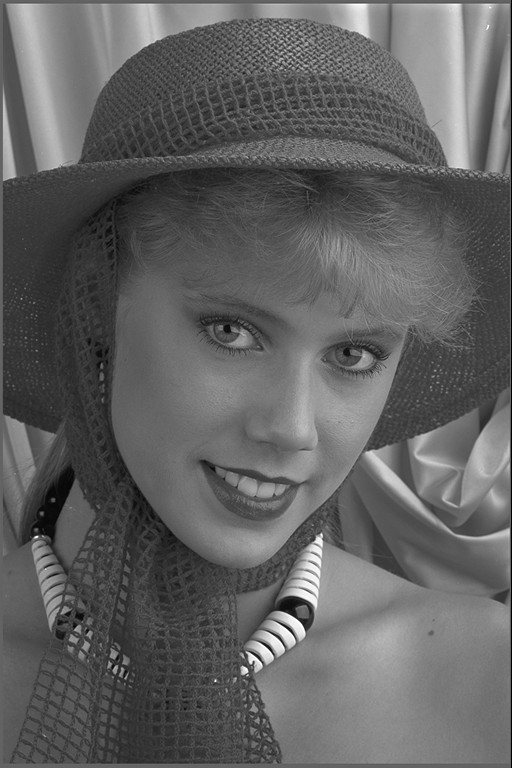
\includegraphics[width=.7\linewidth]{./out/kodim04_Red_Riding_Hood_Y}}
            \caption{image originale}\label{Fig:peppersY-modif-10}
        \end{minipage}\hfill
        \begin{minipage}{0.48\textwidth}
            \centering
            \fbox{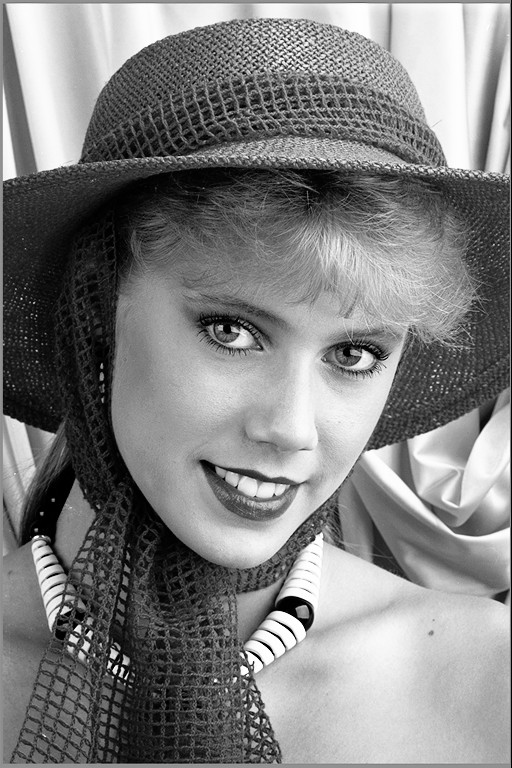
\includegraphics[width=.7\linewidth]{./out/kodim04_Red_Riding_Hood_Y_egal}}
            \caption{image modifiée}\label{Fig:peppersY-modif-50}
        \end{minipage}
    \end{figure}
    On obtient cet histogramme :
    % insert peppersY-modif-'k' with k = 10, 50, -30
    \begin{figure}[!htb]
        \begin{minipage}{0.48\textwidth}
            \centering
            \fbox{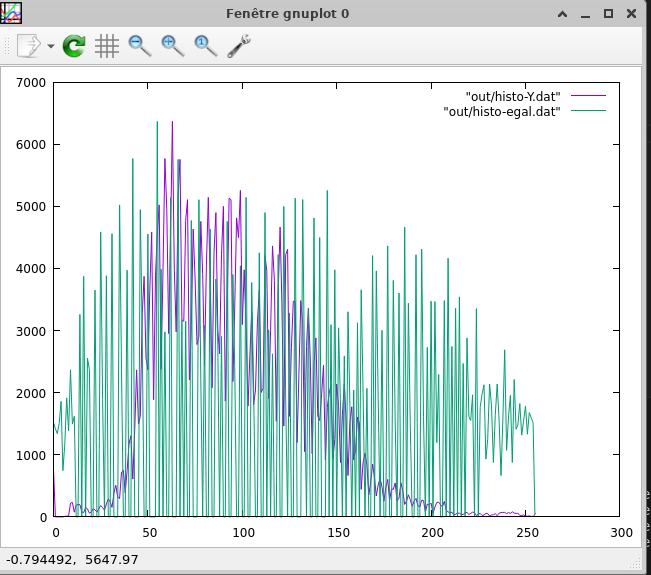
\includegraphics[width=.7\linewidth]{./out/histo-egal}}
            \caption{image contrastée}\label{Fig:peppersY-modif-10}
        \end{minipage}
    \end{figure}

    On constate que ces deux histogrammes n'ont presque rien avoir et que
    celui de l'image modifiée a une bien meilleure répartition de niveaux de gris.

    \newpage

    \section{Lissage d'une image contrastée}\label{sec:5}

    \subsection{Filtre gaussien}\label{subsec:4.2}

    On crée un programme \texttt{filtre\_gaussien.cpp} qui prend en entrée une image et un masque de filtrage.
    Le programme retourne une image filtrée. On utilisera ici $n=3$.

    On applique le programme sur l'image originale avec un masque de 3x3 : % insert images
    \begin{figure}[!htb]
        \begin{minipage}{0.48\textwidth}
            \centering
            \fbox{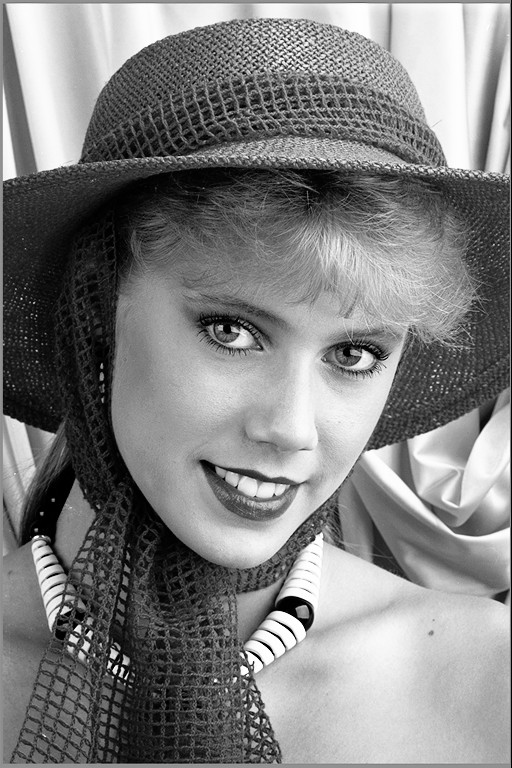
\includegraphics[width=.7\linewidth]{./out/kodim04_Red_Riding_Hood_Y_egal}}
            \caption{Image originale}\label{Fig:peppers-grey-2}
        \end{minipage}\hfill
        \begin{minipage}{0.48\textwidth}
            \centering
            \fbox{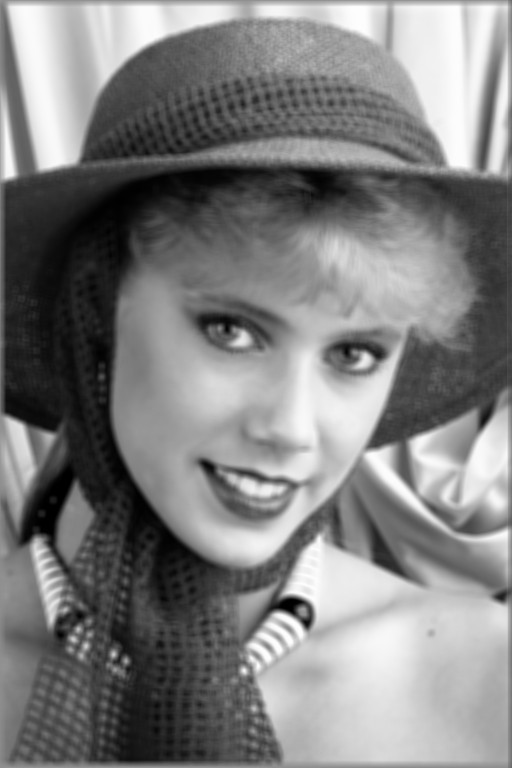
\includegraphics[width=.7\linewidth]{./out/gauss}}
            \caption{Image filtrée}\label{Fig:filtre-gaussien-peppers-grey}
        \end{minipage}
    \end{figure}

    L'histogramme obtenu est :
    \begin{figure}[!htb]
        \begin{minipage}{0.48\textwidth}
            \centering
            \fbox{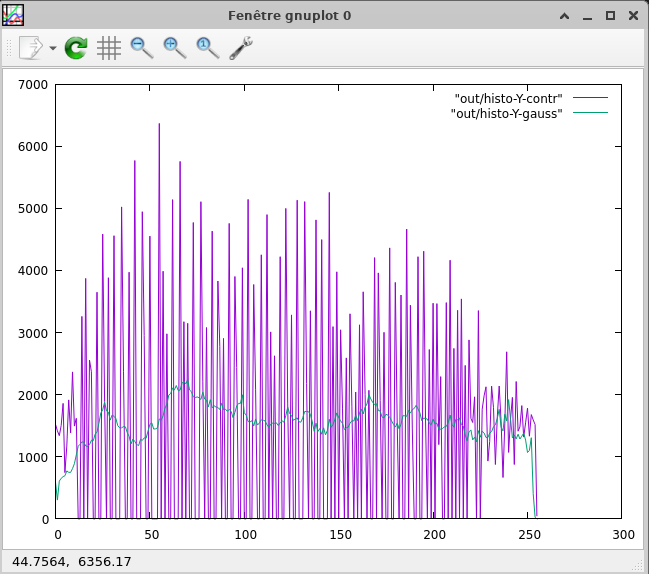
\includegraphics[width=.7\linewidth]{./out/histo-gauss}}
            \caption{Histogrammes}\label{Fig:peppers-grey-2}
        \end{minipage}
    \end{figure}

    On voit très clairement qu'après application du filtre gaussien, il y a une bien meilleure 
    stabilité dans la répartition des niveaux de gris.


\end{document}